\documentclass[../teoria.root.tex]{subfiles}

\begin{document}
\section{Conjuntos}
Un conjunto es una colección de elementos, y se denota usando llaves.
Se pueden declarar de 2 formas:
\begin{itemize}
    \item Extensión: Dando la lista de todos los elementos que pertenecen
          \[ X = \{a, b, c \} \]
          \[ Y = \{ x, \{y\}, \{x,z\} \} \]
          \[ \emptyset = \{\} \]
          \subitem Pseudoextensión: Dando una lista de elementos infinita
          \[ \Z = \{ \dots,-3,-2,-1,0,1,2,3,\dots \} \]
    \item Comprensión: Dando una descripción de cada elemento
          \[ \Q = \left\{\frac{a}{b},\ a,b \in \Z \right\}\]
\end{itemize}

Existen dos conjuntos especiales:
\begin{itemize}
    \item $U$, "Conjunto de referencia", que contiene todos los elementos de todos los conjuntos
          \[ \text{$U$ es $\R$};\ X = \{ x \in \R: 1 \leq x \leq 2 \} = [ 1, 2 ] \]
          \[ \text{$U$ es $\N$};\ Y = \{ y \in \N: 1 \leq x \leq 2 \} = \{ 1, 2\} \]
    \item $\emptyset$, "Conjunto vacio", que no contiene elementos
\end{itemize}

Los elementos de un conjunto se denotan usando el símbolo $\in$ ("pertenece")
y los que \textit{no}, se denotan $\notin$ ("no pertenece").
Todos los elementos o pertenecen a un conjunto, o no.
\begin{align*}
    a,b & \in X    \\
    d   & \notin X
\end{align*}
\[
    \forall x
    \text{ cumple solo una de }
    \left.
    \begin{array}{rl}
        x & \in A    \\
        x & \notin A
    \end{array}
    \right]
    \text{excl.}
\]

Un conjunto jamas se pertenece a si mismo
\[ X \notin X \]
Los elementos pueden aparecer en cualquier orden, y no importa si hay elementos repetidos
\begin{align*}
    \{ 1, 1\cdot1, 1+0 \} & = \{ 1 \}            \\
    \{ 1, 2, 3 \}         & = \{ 3, 2, 1 \}      \\
    \frac{1}{2}           & = \frac{2}{4} \in \Q
\end{align*}


\subsection{Subconjuntos}

\begin{figure}
    \centering
    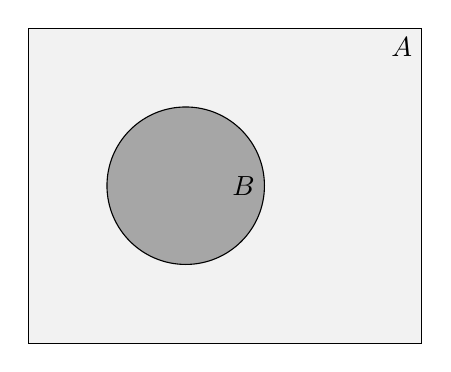
\begin{tikzpicture}
        \draw[fill=gray!10] (-2,-2) rectangle (3,2) node[anchor=north east] {$A$};
        \draw[fill=gray!70] (1,0) arc(360:0:1) node[anchor=east] {$B$};
    \end{tikzpicture}
    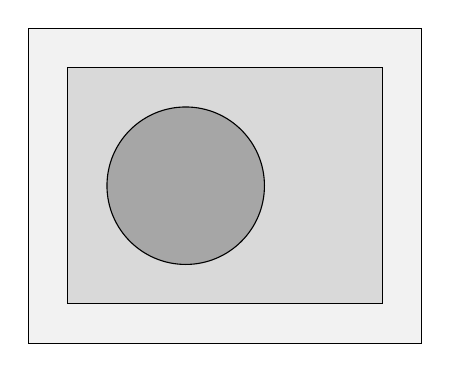
\begin{tikzpicture}
        \draw[fill=gray!10] (-2,-2) rectangle (3,2) node[anchor=north east] {$\C$};
        \draw[fill=gray!30] (-1.5,-1.5) rectangle (2.5,1.5) node[anchor=north east] {$\R$};
        \draw[fill=gray!70] (1,0) arc(360:0:1) node[anchor=east] {$\Q$};
    \end{tikzpicture}
    \caption{
        Podemos representar $B \subseteq A$ graficamente como una figura ($B$) dentro de otra ($A$).
        Un ejemplo real serian los numeros racionales,
        que son contenidos dentro de los reales, que son contenidos dentro de los complejos ($\Q \subseteq \R \subseteq \C$).
    }
\end{figure}

Se denota con el simbolo "$\subseteq$" que todo elemento de un conjunto está presente dentro de otro conjunto.
Mejor dicho, $B \subseteq A$ denota: No hay $e \in B$ que cumpla $e \notin A$; lo que implica que aunque $B$ no tenga
elementos ($B = \emptyset$), $B$ es un subconjunto de $A$
\begin{align*}
    A               & = \{ 1, 2, 3 \}                        \\
    B               & = \{ 1, 2 \}                           \\
    B               & \subseteq A                            \\
    \emptyset       & \subseteq A, B                         \\
    A               & \subseteq A                            \\
    \N \subseteq \Z & \subseteq \Q \subseteq \R \subseteq \C \\
\end{align*}
Si hubiese aun que sea \textit{un} solo elemento en $B$ que no perteneciese a $A$, se denota usando "$\nsubseteq$"
\begin{align*}
    A & = \{ 1, 2, 3 \}          \\
    B & = \{ 1, 2, \textbf{4} \} \\
    B & \nsubseteq A
\end{align*}

\subsubsection{Unión e intersección}
Se puede crear subconjuntos a partir de otros conjuntos.
Se denota $A \cup B$ un conjunto que esta compuesto por todos los elementos de $A$ y $B$,
y $A \cap B$ un conjunto que esta compuesto por los elementos que $A$ y $B$ tienen en común
\[ A \cup B = \{ u \in U / u \in A \lor u \in B \} \]
\[ A \cap B = \{ u \in U / u \in A \land u \in B \} \]
\begin{align*}
    A & =  \{ 1, 2, 3, 4 \} & A \cup B & = \{ 1, 2, 3, 4, 5, 6 \} \\
    B & =\{ 1, 2, 5, 6 \}   & A \cap B & = \{ 1, 2 \}
\end{align*}
% Diagrama de Venn

\subsubsection{Complemento}
Se dentota $A^c$ al \textit{complemento de $A$}, que es un conjunto compuesto por
todos los elementos de $U$, excepto aquellos que pertenecen a $A$.
\[ A^c = \{ a \in U / a \notin A \} \]
\begin{align*}
    U & =  \{1, 2, 3\} & A^c        & = \{3\}            \\
    A & = \{1, 2\}     & A \cup A^c & = \{1, 2, 3\} = U  \\
      &                & A \cap A^c & = \{\} = \emptyset
\end{align*}

\subsubsection{Diferencia}
Dados dos conjuntos $A$ y $B$, se denota $A - B$ al conjunto compuesto por todos
los elementos de $A$, execpto aquellos que esten presentes en $B$. Tambien puede
interpretarse como "todos los elementos de $A$ que tambien esten presentes en $B^c$"
\[ A - B = A \cap B^c = \{ u \in U / u \in A \land u \notin B \} \]
\begin{align*}
    A & = \{1, 2, 3\}    & A - B         & = \{3\}     \\
    B & = \{1, 2, 4\}    & B - A         & = \{4\}     \\
    U & = \{1, 2, 3, 4\} & A - A         & = \emptyset \\
      &                  & A - A^c       & = A         \\
      &                  & A - \emptyset & = A         \\
      &                  & A - U         & = \emptyset
\end{align*}

\subsubsection{Diferencia simétrica}
Tambien nombrada "ó exclusivo". Dados dos conjuntos $A$ y $B$, se denota $A \triangle B$
al conjunto compuesto por todos los elementos de $A$ que no esten presentes en $B$ y vice versa.
\begin{align*}
    A \triangle B & = \{u \in U / (u \in A \land u \notin B) \lor (u \notin A \land u \in B) \} \\
                  & = (A - B) \cup (B - A)
\end{align*}
\begin{align*}
    A & = \{1, 2, 3\} & A \triangle B         & = \{3, 4\}  \\
    B & = \{1, 2, 4\} & B \triangle A         & = \{3, 4\}  \\
      &               & A \triangle \emptyset & = A         \\
      &               & A \triangle U         & = \emptyset
\end{align*}
\subsubsection{Producto cartesiano}
Dados dos conjuntos, $A$ y $B$, se denota $A \x B$ al conjunto de todos los pares $(a, b)$ con $a \in A$ y $a \in B$
\[ A \x B = \{(a_1, b_1), (a_1, b_2), (a_1, b_3), \dots, (a_1, b_m), (a_2, b_1), (a_2, b_2), \dots, (a_n, b_m)\} \]
\begin{align*}
    A & = \{a, b\} & A \x B                             & \neq B \x A                          \\
    B & = \{1, 2\} & \{(a, 1), (a, 2), (b, 1), (b, 2)\} & = \{(1, a), (1, b), (2, a), (2, b)\} \\
      &            &
\end{align*}

\subsection{Tablas de verdad}
\subsection{Relaciones}


\end{document}